%; whizzy paragraph -pdf xpdf -latex ./whizzypdfptex.sh
%; whizzy-paragraph "^\\\\begin{frame}"
% latex beamer presentation.
% platex, latex-beamer でコンパイルすることを想定。 

%     Tokyo Debian Meeting resources
%     Copyright (C) 2009 Junichi Uekawa

%     This program is free software; you can redistribute it and/or modify
%     it under the terms of the GNU General Public License as published by
%     the Free Software Foundation; either version 2 of the License, or
%     (at your option) any later version.

%     This program is distributed in the hope that it will be useful,
%     but WITHOUT ANY WARRANTY; without even the implied warranty of
%     MERCHANTABILITY or FITNESS FOR A PARTICULAR PURPOSE.  See the
%     GNU General Public License for more details.

%     You should have received a copy of the GNU General Public License
%     along with this program; if not, write to the Free Software
%     Foundation, Inc., 51 Franklin St, Fifth Floor, Boston, MA  02110-1301 USA

\documentclass[cjk,dvipdfmx,12pt]{beamer}
\usetheme{Tokyo}
\usepackage{monthlypresentation}

%  preview (shell-command (concat "evince " (replace-regexp-in-string "tex$" "pdf"(buffer-file-name)) "&"))
%  presentation (shell-command (concat "xpdf -fullscreen " (replace-regexp-in-string "tex$" "pdf"(buffer-file-name)) "&"))
%  presentation (shell-command (concat "evince " (replace-regexp-in-string "tex$" "pdf"(buffer-file-name)) "&"))

%http://www.naney.org/diki/dk/hyperref.html
%日本語EUC系環境の時
\AtBeginDvi{\special{pdf:tounicode EUC-UCS2}}
%シフトJIS系環境の時
%\AtBeginDvi{\special{pdf:tounicode 90ms-RKSJ-UCS2}}

\title{東京エリア Debian 勉強会}
\subtitle{資料}
\author{上川 純一 dancer@debian.or.jp\\IRC nick: dancerj}
\date{2009年4月18日}
\logo{
\includegraphics[width=8cm]{image200607/openlogo-light.eps}}


\begin{document}

\frame{\titlepage{}}

\emtext{設営準備にご協力ください}

\begin{frame}{今日の参加の目標}
\begin{itemize}
 \item 前田: ocaml 勉強しに来ました
 \item きたはら: ocamlって何ですか
 \item 中尾: java policy 勉強しにきました
 \item 山本: 飲みにきました
 \item 吉田@板橋: poken個人情報漏洩しにきた
 \item まとはら: 誰かDebianで動くoutliner のよいソフトをおしえてください
 \item あけど: emacs を使えるようになりたい。なんか紹介してください。
       MacOSの消し方を知りたい。 emacs -nw
 \item 高橋(仮): poken を受けとりに着た
 \item やまだ: DDTP: 作業効率よくなるネタがあるとうれしい。omegat?
 \item 小川: poken を渡しに来た。
 \item 日比野: ocaml の入門ぷりをチェックしたい。
\end{itemize}
\end{frame}

\section{}
\begin{frame}{前回考えていた今回のテーマ}
\begin{itemize}
 \item 事前課題: 「やまねさんの開発効率を上げる方法を提案してください。」
 \item 藤澤さん: 連載GXP: ITPしてみました。
 \item John: I made a clozurecl package!
 \item やまね: 俺の開発効率をあげてください session。
\end{itemize}
\end{frame}


\begin{frame}
 \frametitle{Agenda}
\begin{minipage}[t]{0.45\hsize}
  \begin{itemize}
  \item 注意事項
	\begin{itemize}
	 \item 飲食禁止
	 \item 政治/宗教/営利活動禁止
	\end{itemize}
  \item 最近あったDebian関連のイベント報告
	\begin{itemize}
	 \item 前回の勉強会
	 \item OSC
	 \item Ubuntu オフラインミーティング@秋葉原
	 \item Linux Consortium 10 years event
	 \item Hack Cafe
	\end{itemize}
 \end{itemize}
\end{minipage} 
\begin{minipage}[t]{0.45\hsize}
 \begin{itemize}
  \item Debian Java policy について
  \item Debian 開発のワークフローについて語る会
  \item ocaml勉強はじめました
 \end{itemize}
\end{minipage}
\end{frame}

\section{最近}

\begin{frame}
 \frametitle{2009年03月}
\begin{minipage}[t]{0.45\hsize}
  \begin{itemize}
  \item 注意事項
	\begin{itemize}
	 \item ?
	\end{itemize}
  \item 最近あったDebian関連のイベント報告
	\begin{itemize}
	 \item 前回の勉強会
	 \item OSC
	 \item Ubuntu オフラインミーティング@秋葉原
	 \item Linux Consortium 10 years event
	 \item Hack Cafe
	\end{itemize}
 \end{itemize}
\end{minipage} 
\begin{minipage}[t]{0.45\hsize}
 \begin{itemize}
  \item Debian クイズ
  \item 研究室のソフトウェアを Debian パッケージにしてみる
  \item Debian での Common Lispプログラミング環境
 \end{itemize}
\end{minipage}
\end{frame}

\begin{frame}{Hack Cafe}

毎週水曜日、週に一回東京のどっかのカフェでハック。

\end{frame}

\section{DWN quiz}
\begin{frame}{Debian 常識クイズ}

Debian の常識、もちろん知ってますよね?
知らないなんて恥ずかしくて、知らないとは言えないあんなことやこんなこと、
みんなで確認してみましょう。

今回の出題範囲は\url{debian-devel-announce@lists.debian.org} に投稿された
内容とDebian Project Newsからです。

\end{frame}

\subsection{問題}
%; whizzy-master ../debianmeetingresume200904.tex
% $B0J>e$N@_Dj$r$7$F$$$k$?$a!"$3$N%U%!%$%k$G(B M-x whizzytex $B$9$k$H!"(Bwhizzytex$B$,MxMQ$G$-$^$9!#(B

 \santaku
 {4$B7n(B9$BF|$K%"%C%W%G!<%H$5$l$?(B etch $B$N%P!<%8%g%s$O(B?}
 {4.0r8}
 {4.0beta8}
 {etch-a-sketch}
 {A}
{}

 \santaku
 {4$B7n(B11$BF|$K%"%C%W%G!<%H$5$l$?(B lenny $B$N%P!<%8%g%s$O(B?}
 {5.0r1}
 {5.0.1}
 {lenny++}
 {B}
{}

 \santaku
 {Debian.org DPL $B$K$J$C$?$N$O!)(B}
 {Stefano Zacchiroli}
 {Steve McIntyre}
 {Nobuhiro Iwamatsu}
 {B}
{}

 \santaku
 {Debian JP Leader $B$K$J$C$?$N$O(B?}
 {Kei Hibino}
 {Hiroyuki Yamamoto}
 {Nobuhiro Iwamatsu}
 {C}
{}

 \santaku
 {Debian $B$G?7$7$/DI2C$5$l$?%"!<%-%F%/%A%c$O!)(B}
 {GNU/kFreeBSD i386/amd64}
 {GNU/kMinix-3.0 i386/amd64}
 {GNU/kOpenDarwin i386/amd64}
 {A}
{}


\begin{frame}{2009年計画}

{\scriptsize
 \begin{enumerate}
  \item 新年の企画 (アンサンブル荻窪開催)
  \item OSC Tokyo
  \item VAIO P インストール記録、
	カーネル読書会 ディストリビューション大集合(小林さん)(東京大学?)
  \item Git Handson (岩松)(あんさんぶる荻窪?)
  \item 家Debianサーバ vs 職場のネットワーク(千代田区都立図書館?\footnote{\url{http://www.library.chiyoda.tokyo.jp/}})
  \item Asterisk (東京大学?)
  \item スペインにて開催
  \item Debconf報告会
  \item OSC Fall?
  \item udev + HAL
  \item 3D graphics 開発 
  \item Debian サーバ+VMware + 各種OS、
	他の仮想化ツール(vserver etc.)、
	忘年会
 \end{enumerate}
}
\end{frame}

\emtext{Debian Java}

\emtext{Debian で Ocaml 使ってみた}

\begin{frame}{Ocamlはじめてみました}

ocaml 使われている。 advi とか unison とか重要なパッケージが ocaml でか
 かれているんだけど、何がかかれているのかまったく理解できない。

ocaml がまったく理解できないのはまずいので何冊か図書館から本借りてきて読
 むことにした。読むだけではやるきが出ないので今日発表することにしたぜ。
 
\end{frame}

\begin{frame}[containsverbatim]{ocaml の普及度}

\begin{commandline}
$ apt-cache search ocaml | wc -l 
224
\end{commandline}
\end{frame}

\begin{frame}{emacs での利用方法}

tuareg-mode というのがあるよ。

tuareg-run-ocaml でインタラクティブに実行

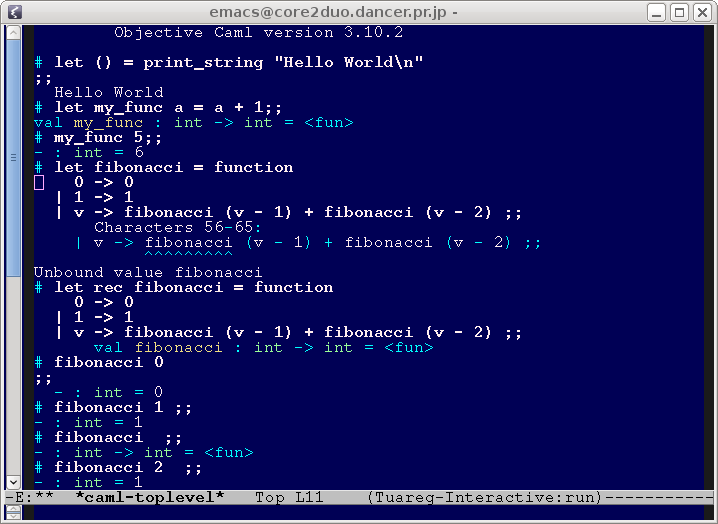
\includegraphics[width=0.9\hsize]{image200904/tuareg-interactive.png}

\end{frame}

\begin{frame}[containsverbatim]{インストール}
\begin{commandline}
# apt-get install tuareg-mode ocaml-native-compilers ocaml-interp ocaml
\end{commandline}
\end{frame}

\begin{frame}[containsverbatim]{とりあえずコード書いてみた}
\begin{commandline}
# 1 + 2 ;;
- : int = 3
\end{commandline}
\end{frame}


\begin{frame}[containsverbatim]{とりあえずコード書いてみた}
\begin{commandline}
let rec fibonacci = function
    0 -> 0
  | 1 -> 1
  | v -> fibonacci (v - 1) + fibonacci (v - 2)

let () = print_int (fibonacci 40); print_newline ()
\end{commandline}
\end{frame}


\begin{frame}{コンパイラでコンパイルしてみる}

\begin{tabular}{|p{7em}|p{8em}|p{8em}|}
 \hline
 & ネイティブコンパイルされた & 中間言語にコンパイルされている\\
 \hline
ネイティブコンパイル結果を出力 &
ocamlopt.opt & ocamlopt\\
 \hline
中間言語を出力 &
ocamlc.opt & ocamlc \\
 \hline
\end{tabular}
\end{frame}

\begin{frame}{fibonacciでとりあえず処理能力を調べてみた}

fibonacci(40)を求めてみた。
再帰アルゴリズムで、C、ocamlopt、ocamlを比較。
\begin{itemize}
 \item C: 2.325s
 \item ocamlopt: 2.933s
 \item ocaml: 14.544s
\end{itemize}
\end{frame}

\begin{frame}{}

先はまだ長そう

\end{frame}

\begin{frame}
\begin{enumerate}
 \item 各自の「私のDebian開発ワークフロー」を紹介してください。
\end{enumerate}
\end{frame}

{\footnotesize
%; whizzy-master ../debianmeetingresume200904.tex
% $B0J>e$N@_Dj$r$7$F$$$k$?$a!"$3$N%U%!%$%k$G(B M-x whizzytex $B$9$k$H!"(Bwhizzytex$B$,MxMQ$G$-$^$9!#(B

\begin{prework}{$B>e@n=c0l(B}
\preworksection{$B;d$N(BDebian$B%o!<%/%U%m!<(B}

$B%P%0%l%]!<%H$rFI$s$G$+$i(B($B0J2<N,(B)

\preworksection{$B$3$&2~A1$7$?$$(B}

$BA4%"!<%-%F%/%A%c$G$N%S%k%I$H%F%9%H$r<+F02=$7$?$$!#(B

\end{prework}

\begin{prework}{$B$^$($@$3$&$X$$(B}
\preworksection{$B;d$N(BDebian$B%o!<%/%U%m!<(B}

ganttproject$B$r=i$a$F(BITP$B$7$F$+$i;_$^$C$?$^$^!#(B

\preworksection{$B$3$&2~A1$7$?$$(B}

$B2HDm$H;E;v$K1F6A$5$l$:$K%Q%C%1!<%8%a%s%F%J%s%9$G$-$k$h$&$K$7$F$$$-$?$$!#(B

\end{prework}


% \begin{prework}{$BL>A0(B}
% \preworksection{$B;d$N(BDebian$B%o!<%/%U%m!<(B}
% \preworksection{$B$3$&2~A1$7$?$$(B}
% \end{prework}
% $B0J2<$KF1MM$N%F%s%W%l!<%H$GDI2C$9$k!#(B


\begin{prework}{$B>.@n?-0lO:(B}
\preworksection{$B;d$N:n6H4D6-$K$D$$$F(B}
$B2q<R$G$O(B Ubuntu 8.04.1 Desktop $B$r%$%s%9%H!<%k$7$?%G%9%/%H%C%W(BPC$B$G!$(B
$B2H$G$O(B Ubuntu 8.10 $B$r%$%s%9%H!<%k$7$?(B Thinkpad X61 $B$r;H$C$F!$(B
$B3+H/$dF|!9$N6HL3$J$I$r$3$J$7$F$$$^$9!%(B
$BA4A3(B Debian $B$8$c$J$$$N$G$9$,!$(BRuby on Rails $B$J$N$G!$(B
Ruby $B$N(B Version $B$,$"$o$J$$$N$G!$(BUbuntu $B;H$C$F$$$^$9!%(B

GW$BCf$K(B Thinkpad $B$K(B Lenny $BF~$l$kM=Dj$G$9!%(B
$B2q<R$N%5!<%P72$b!$(BDebian $B$K$7$?$$$J$H!$$$$m$$$mLO:wCf$G$9!%(B

\end{prework}

\begin{prework}{$B;3K\9@G7(B}
\preworksection{$B;d$N(BDebian$B%o!<%/%U%m!<(B}

$B%Q%C%1!<%82=$7$?$$%=%U%H%&%'%"$r8+$D$1$?$i!"$^$:<+J,<+?HMQ$NLnNI%Q%C%1!<%8$r:n$j!";n$7$^$9!#<!$KBg;(GD$K%i%$%;%s%9$r3NG'$7!"NI$5$2$J$i!"<+J,$K3e$rF~$l$k$?$a(B ITP $B$7$^$9(B($B>P(B)$B!#$=$l$+$i%3!<%I$J$I!"5;=QE*$J8!F$$KF~$j$^$9(B ($B$3$3$G:C@^$7$?$b$N$b$$$/$D$"$k$N$d$i!D(B)$B!#$5$i$K%3%T!<%i%$%H$d%i%$%;%s%9$N@:::$r$7!"(Bdebian/copyright $B$r40@.$5$;$^$9!#<!$K;d$K$H$C$F$H$F$bFq4X$N(B($B>P(B)$B1Q8l$N%I%-%e%a%s%H$r$D$1$F!"(Bpbuilder $B$G%S%k%I$7$^$9!#:G8e$K(B mentors.debian.net $B$X$N%"%C%W%m!<%I$H(B mentors@org ML$B!"$*$h$S(B debian-develop@jp ML $B$K%a!<%k$rEj$2$F%9%]%s%5!<C5$7$r$7$^$9!#0J>e!#(B

\preworksection{$B$3$&2~A1$7$?$$(B}

$B$_$s$J$,;H$C$F$$$kJ8;z%3!<%I$d(B locale $B$r(B UTF-8 $B$KE}0l$7$?$$!#(B

\end{prework}


}


\begin{frame}{Debconf 2009}
\begin{itemize}
 \item スペイン参加
 \item 飛行機代20万弱
 \item 7/23-7/30
 \item 優待つき事前参加登録締切りは4月15日まで、それ以降の参加登録は 300
       euro 以上必要。
 \item \url{http://debconf9.debconf.org/register.xhtml}
\end{itemize}
\end{frame}

\begin{frame}{宴会場所}
\begin{itemize}
 \item 宴会場所\\
       本日の宴会は「はなの舞」です。\\
       21:00 開始です。
       参加者は1Fに集合して全員で移動しましょう。
 \item 片付け\\
       部屋を片付けるのにご協力ください。
\end{itemize}
\end{frame}

\end{document}

;;; Local Variables: ***
;;; outline-regexp: "\\([ 	]*\\\\\\(documentstyle\\|documentclass\\|emtext\\|section\\|begin{frame}\\)\\*?[ 	]*[[{]\\|[]+\\)" ***
;;; End: ***
